SKA will be the world's largest radio-telescope. It will be located in two different geographical areas: South Africa and Australia/New Zealand. It will be
constructed in different phases: SKA1 (phase 1 2018-2023) and SKA2 (phase 2
2023-2033). The development will be deployed using two different pathfinders
existing on each place (MeerKAT in South Africa \cite{ska:meerkat} and ASKAP in Australia \cite{ska:askap}).  
SKA1 starts in 2018 and it is intended to cover the ~10\% of
the total area at low and mid frequencies by 2023. SKA2 has
the goal to get the full array working at low and mid frequencies by 2030.

There will be two different SKA facility locations depending on the frequency
range for the sky observations. A common factor in both of them, is the high level of synchronisation accuracy due to the huge number of antennas needed.
More information can be found in  \cite{ska:baseline_description_v2}. Under
this context and as \cite{HUANG201727} suggests, the computer network in
astrophysics science is one of the most important elements and determines key
aspects such as system performance.

\subsection{SKA Telescope Network} \label{subsec:ska-telescope}

The SKA Telescope uses different types of networks to guarantee a proper
operation of the infrastructure. These networks are described briefly in
Figure \ref{fig:ska_net_arch1}. The design of the network corresponds to the
Signal and Data Transport (SaDT) element \cite{ska:sadt_website} and it
includes all the necessary hardware and software for the transmission of data and
information between the elements of SKA. SADT also contains details about
the provision of timing which is critical for interferometry.  The data network
includes the Digital Data Back-haul (DDBH) that transports signals from the
radio telescopes to the Central Signal Processor (CSP), and data products from
the CSP to the Science Data Processor (SDP) and from the SDP to the regional
SKA Data Centres. The total data rates are very high, approximately 80 Tb/s for
the DDBH links and another 80Tb/s for the CSP links \cite{ska:consortia-news}.
Also covered by the SaDT is the Monitor and Control (M\&C) that transmits and
receives monitoring and control information throughout the system and includes
the Telescope Manager, itself comprised of three logical networks: Production
Network, Engineering Network and Safety Network.

\begin{figure}[H] \centering 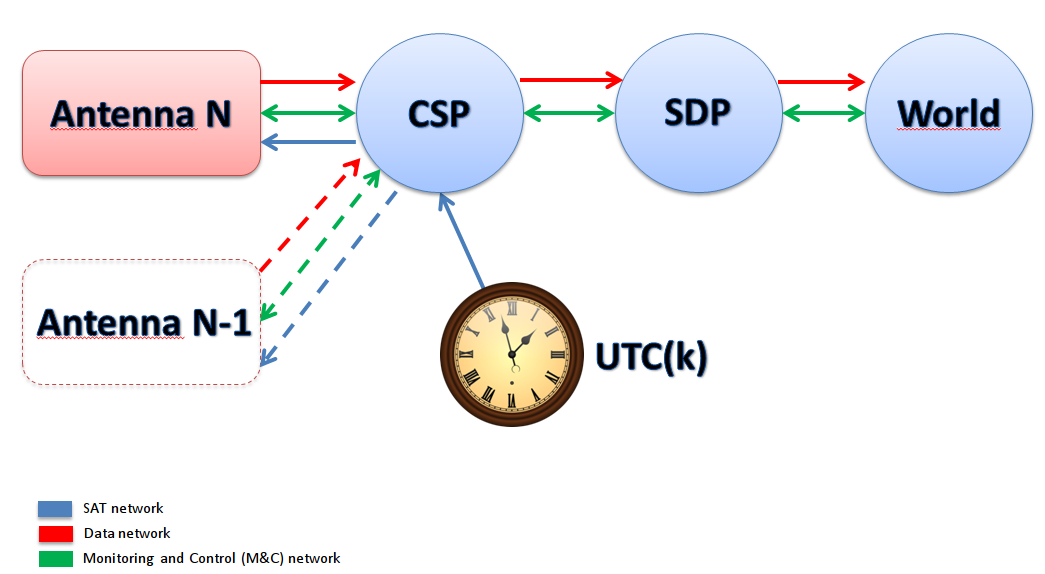
\includegraphics[scale=0.4]{img/ska_network_arch}
	\caption{The SKA Telescope network architecture is composed of three
	networks: the data network (red), the M\&C network (green) and the SAT
	network (blue). An external clock reference, UTC traceable, is provided
	to the whole Telescope elements in order of providing an unique time
	reference.} \label{fig:ska_net_arch1} \end{figure}

The final part of the SaDT is the Synchronisation and Timing (SAT) that
provides frequency and clock signals from a central clock ensemble to all
elements of the system to maintain the same phase information on all receptors, 
timing signals for data identification and time critical activities. 
In order to maintain phase coherence across the array, it is required a short-term 
timing precision of around 1 ps, while  an accuracy of 10 ns for 10 years periods 
becomes mandatory for long-term timing pulsar requirements. 
Timing is critical for the correct SKA functioning to
work as a unified large telescope using a technique known as interferometry.
This contribution focuses on the high accuracy synchronisation method used for
SKA responsible to provide a PPS signal to the critical elements. 

\FloatBarrier
\subsection{High-accuracy timing signals distribution for SKA1}
\label{subsec:ska-distribution}

As determined by SaDT, the SKA Telescope should be able to distribute a common frequency reference to all the antennas in order to provide a unique time reference to register all the events with ultra-high accuracy using timestamps. This task is performed by the SAT element that belongs to SaDT. The SKA timescale is maintained by the central clock ensemble and it is disseminated to the rest of the antennas. These clock ensembles form the fundamental timescale for SKA and will be the basis to perform precise measurements of pulsars and other time-dependent phenomenons. It is important to remark that SaDT uses different mechanisms to achieve frequency dissemination and PPS distribution goals but our contribution only address a suitable candidate solution for the second issue. 
The \cite{paultests} summarises the PPS distribution requirements. As previously presented, it is constrained to 10 ns. However, the UTC realisation error must be bounded below 5 ns and the synchronisation technology only has a 2 ns budget. Based on current SAT network topology, the target specification for the elements of the PPS distribution system provides them an average time better than 2 ns. 

The PPS distribution system will be in charge of delivering its output at the following locations: SKA1-MID with 133 dishes connected to optical fibre links between 120-150 km and SKA1-LOW with 45 stations along 3 spiral arms connected to optical fibre links between 70-80 km. Depending on the frequency offset scheme applied to all SKA1-MID dishes, additional 64 endpoints may be needed in SKA1-MID. By this, the synchronisation network might be increased from 182 to 246 endpoints. These numbers allow to estimate the time transfer network complexity but note that a complete description of the SKA network elements and topology is out of the scope of this contribution.

In addition, SKA1 uses aerial optical fibre networks that are
significantly affected by the large temperature excursion during operation,
presenting variations of more than 20\degree C in desert locations, such as South Africa and Australia. Furthermore, outdoor wind velocities during normal operation could achieve up to 40 km/h, making fibres oscillate and changing their length, forcing to develop a compensation mechanism on real-time during execution. 

As a summary, the SKA Telescope has a quite challenging goal because it imposes a high accuracy synchronisation requirement and also for the dynamic environmental operation conditions of the facility.

Next section describes the WR technology introducing its main features and its different network elements.